\begin{figure}[htbp]
\centering
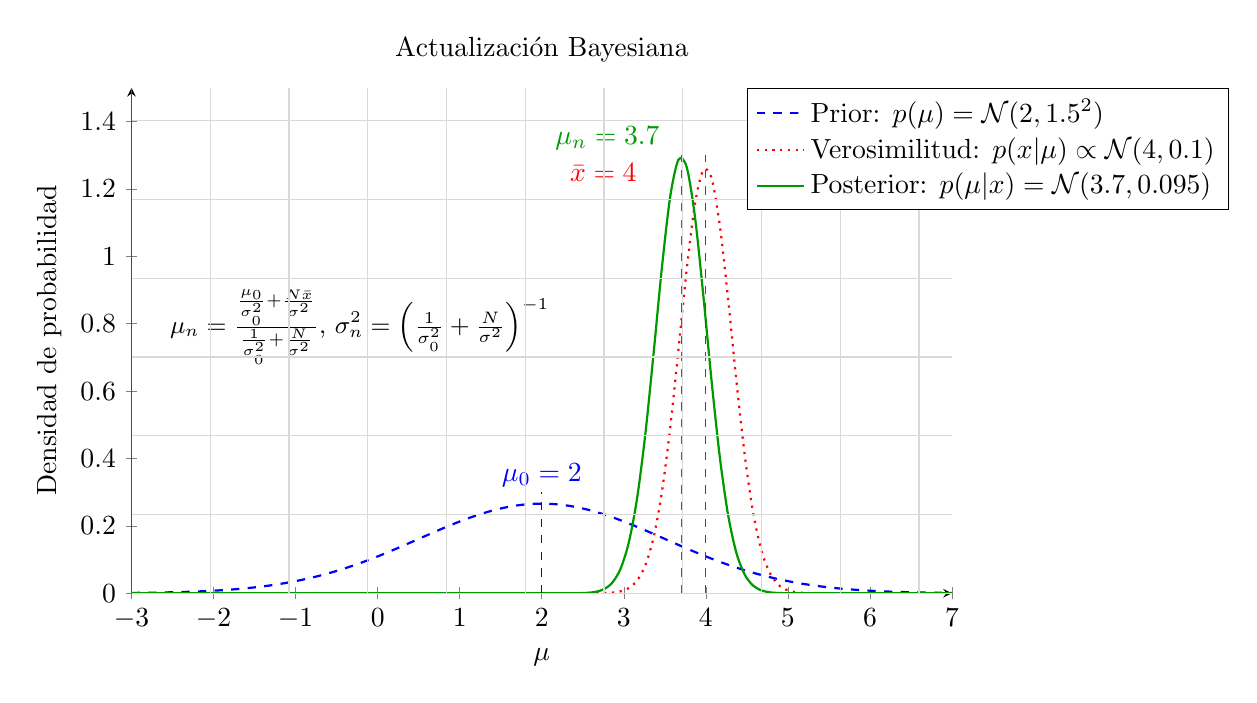
\begin{tikzpicture}
\begin{axis}[
    width=12cm,
    height=8cm,
    axis lines=left,
    xlabel={$\mu$},
    ylabel={Densidad de probabilidad},
    domain=-3:7,
    samples=100,
    smooth,
    title={Actualización Bayesiana},
    legend style={at={(0.75,1.0)}, anchor=north west},
    legend cell align=left,
    ymax=1.5,    % Aumentado para mostrar los picos completos
    scaled y ticks=false
]

% Prior - N(2, 1.5²)
\addplot[thick, blue, dashed] {exp(-(x-2)^2/(2*2.25))/sqrt(2*pi*2.25)};
\addlegendentry{Prior: $p(\mu) = \mathcal{N}(2, 1.5^2)$}

% Likelihood basada en datos con media muestral 4, N=10, sigma=1
\addplot[thick, red, dotted] {exp(-(x-4)^2/(2*0.1))/sqrt(2*pi*0.1)};
\addlegendentry{Verosimilitud: $p(x|\mu) \propto \mathcal{N}(4, 0.1)$}

% Posterior - combinación de prior y likelihood
\addplot[thick, green!60!black] {exp(-(x-3.7)^2/(2*0.095))/sqrt(2*pi*0.095)};
\addlegendentry{Posterior: $p(\mu|x) = \mathcal{N}(3.7, 0.095)$}

% Añadir líneas verticales para las medias
\draw[dashed, blue] (axis cs:2,0) -- (axis cs:2,0.3);
\node[blue] at (axis cs:2,0.35) {$\mu_0=2$};

\draw[dashed, red] (axis cs:4,0) -- (axis cs:4,1.3);
\node[red] at (axis cs:2.75,1.25) {$\bar{x}=4$};

\draw[dashed, green!60!black] (axis cs:3.7,0) -- (axis cs:3.7,1.3);
\node[green!60!black] at (axis cs:2.8,1.35) {$\mu_n=3.7$};

% Añadir fórmulas del posterior con posición ajustada
\node[align=left, anchor=south west, font=\small] at (axis cs:-2.65,0.65) {
$\mu_n = \frac{\frac{\mu_0}{\sigma_0^2} + \frac{N\bar{x}}{\sigma^2}}{\frac{1}{\sigma_0^2} + \frac{N}{\sigma^2}}$, 
$\sigma_n^2 = \left(\frac{1}{\sigma_0^2} + \frac{N}{\sigma^2}\right)^{-1}$
};

\draw[gray!30, thin] (axis cs:-3,0) grid (axis cs:7,1.5);

\end{axis}
\end{tikzpicture}
\caption{Actualización bayesiana de la distribución de $\mu$. Ilustra cómo el conocimiento previo (prior) 
se combina con la evidencia (verosimilitud) para obtener la distribución posterior. En este ejemplo, 
asumimos un prior $\mathcal{N}(2, 1.5^2)$, datos con media muestral $\bar{x}=4$ ($N=10$, $\sigma^2=1$), 
resultando en un posterior $\mathcal{N}(3.7, 0.095)$ que se desplaza hacia la evidencia pero con menor varianza que ambas distribuciones originales.}
\label{fig:bayesian_update}
\end{figure}